%Notes by Harsh Mistry 
%CS240
%based on Template from : https://www.cs.cmu.edu/~ggordon/10725-F12/template.tex

\documentclass{article}
\setlength{\oddsidemargin}{0.25 in}
\setlength{\evensidemargin}{-0.25 in}
\setlength{\topmargin}{-0.6 in}
\setlength{\textwidth}{6.5 in}
\setlength{\textheight}{8.5 in}
\setlength{\headsep}{0.75 in}
\setlength{\parindent}{0 in}
\setlength{\parskip}{0.1 in}
\usepackage{amsfonts,graphicx, amssymb}
\usepackage[fleqn]{amsmath}
\usepackage{fixltx2e}
\usepackage{tikz}
\usepackage{color}
\usepackage{tcolorbox}
\usepackage{lipsum}
\usepackage{listings}
\usepackage{scrextend}
\usepackage{graphicx}
\graphicspath{ {images/} }
\tcbuselibrary{skins,breakable}
\usetikzlibrary{shadings,shadows}
\newcounter{lecnum}
\renewcommand{\thepage}{\thelecnum-\arabic{page}}
\renewcommand{\thesection}{\thelecnum.\arabic{section}}
\renewcommand{\theequation}{\thelecnum.\arabic{equation}}
\renewcommand{\thefigure}{\thelecnum.\arabic{figure}}
\renewcommand{\thetable}{\thelecnum.\arabic{table}}
\newcommand{\lecture}[4]{
   \pagestyle{myheadings}
   \thispagestyle{plain}
   \newpage
   \setcounter{lecnum}{#1}
   \setcounter{page}{1}
   
   
%Info Box 
   \begin{center}
   \framebox{
      \vbox{\vspace{2mm}
    \hbox to 6.28in { {\bf CS 240 - Data Structures and Data Management
	\hfill Spring 2017} }
       \vspace{4mm}
       \hbox to 6.28in { {\Large \hfill Lecture #1: #2  \hfill} }
       \vspace{2mm}
       \hbox to 6.28in { {\it Lecturer: #3 \hfill Notes By: #4} }
      \vspace{2mm}}
   }
   \end{center}
   
   \markboth{Lecture #1: #2}{Lecture #1: #2}



 
}

\renewcommand{\cite}[1]{[#1]}
\def\beginrefs{\begin{list}%
        {[\arabic{equation}]}{\usecounter{equation}
         \setlength{\leftmargin}{2.0truecm}\setlength{\labelsep}{0.4truecm}%
         \setlength{\labelwidth}{1.6truecm}}}
\def\endrefs{\end{list}}
\def\bibentry#1{\item[\hbox{[#1]}]}

\newcommand{\fig}[3]{
			\vspace{#2}
			\begin{center}
			Figure \thelecnum.#1:~#3
			\end{center}
	}
	
\newcommand{\pipe}{\(\mid\)}
\newcommand{\ctr}{\(\wedge\)}

\newtheorem{theorem}{Theorem}[lecnum]
\newtheorem{lemma}[theorem]{Lemma}
\newtheorem{ex}[theorem]{Example}
\newtheorem{proposition}[theorem]{Proposition}
\newtheorem{claim}[theorem]{Claim}
\newtheorem{corollary}[theorem]{Corollary}
\newtheorem{definition}[theorem]{Definition}
\newenvironment{proof}{{\bf Proof:}}{\hfill\rule{2mm}{2mm}}
\newcommand\E{\mathbb{E}}

%color definitions :
\definecolor{darkred}{rgb}{0.55, 0.0, 0.0}
\definecolor{lightcoral}{rgb}{0.94, 0.5, 0.5}
\definecolor{tomato}{rgb}{1.0, 0.39, 0.28}
\definecolor{lightgray}{rgb}{.9,.9,.9}
\definecolor{darkgray}{rgb}{.4,.4,.4}
\definecolor{purple}{rgb}{0.65, 0.12, 0.82}
\definecolor{lightgreen}{rgb}{0.56, 0.93, 0.56}
\definecolor{darkgreen}{rgb}{0.0, 0.2, 0.13}
\definecolor{limegreen}{rgb}{0.2, 0.8, 0.2}
\definecolor{lightblue}{rgb}{0.68, 0.85, 0.9}
\definecolor{darkblue}{rgb}{0.0, 0.0, 0.55}


%Environments
\newenvironment{exblock}[1]{%
    \tcolorbox[beamer,%
    noparskip,breakable,
    colback=lightgreen,colframe=darkgreen,%
    colbacklower=limegreen!75!lightgreen,%
    title=#1]}%
    {\endtcolorbox}

\newenvironment{ablock}[1]{%
    \tcolorbox[beamer,%
    noparskip,breakable,
    colback=lightcoral,colframe=darkred,%
    colbacklower=tomato!75!lightcoral,%
    title=#1]}%
    {\endtcolorbox}

\newenvironment{cblock}[1]{%
    \tcolorbox[beamer,%
    noparskip,breakable,
    colback=lightblue,colframe=darkblue,%
    colbacklower=darkblue!75!lightblue,%
    title=#1]}%
    {\endtcolorbox}


%Languages
\lstdefinelanguage{JavaScript}{
  keywords={typeof, new, true, false, catch, function, return, null, catch, switch, var, if, in, while, do, else, case, break},
  keywordstyle=\color{blue}\bfseries,
  ndkeywords={class, export, boolean, throw, implements, import, this},
  ndkeywordstyle=\color{darkgray}\bfseries,
  identifierstyle=\color{black},
  sensitive=false,
  comment=[l]{//},
  morecomment=[s]{/*}{*/},
  commentstyle=\color{purple}\ttfamily,
  stringstyle=\color{red}\ttfamily,
  morestring=[b]',
  morestring=[b]"
}

%Listings
\lstset{
   language=JavaScript,
   backgroundcolor=\color{lightgray},
   extendedchars=true,
   basicstyle=\footnotesize\ttfamily,
   showstringspaces=false,
   showspaces=false,
   numbers=left,
   numberstyle=\footnotesize,
   numbersep=9pt,
   tabsize=2,
   breaklines=true,
   showtabs=false,
   captionpos=b
}


%Start
\begin{document}

\lecture{21, 22, 23}{July 18  - 25, 2017}{Taylor Smith}{Harsh Mistry}

\section{Compression}
\textbf{The problem} : How to store and transmit data?

\subsection*{Judging Encoding Schemes}
Encoding schemes that try to minimize \(\mid C \mid \), the size of the coded text,
perform data compression. We will measure the compression ratio:
$$ \frac{\mid C \mid \cdot \log \mid \sum_C \mid}{\mid S \mid \cdot \log \mid \sum_S \mid} $$

\subsection*{Types of Data Compression}
\textbf{Logical vs. Physical}
\begin{itemize}
\item Logical Compression uses the meaning of the data and only applies
to a certain domain (e.g. sound recordings)
\item Physical Compression only knows the physical bits in the data, not the meaning behind them
\end{itemize}

\textbf{Lossy vs. Lossless}
\begin{itemize}
\item Lossy Compression achieves better compression ratios, but the
decoding is approximate; the exact source text S is not recoverable
\item Lossless Compression always decodes S exactly
\end{itemize}

\subsection*{Encodings}

\begin{definition}
\textbf{Character Encodings: } Standard character encodings provide a matching from the source
alphabet \(\sum_S\) (sometimes called a charset) to binary strings.
\end{definition}

\begin{definition}
\textbf{Variable-Length Codes: } Different key strings have different lengths.
\end{definition}

\subsection*{Decoding}
We need a decoding algorithm mapping \(\sum_C^* \rightarrow \sum_S^*\). A prefix-free code will have a fixed dictionary to support such a mapping. 

\subsection*{Huffman Coding}
\begin{itemize}
\item Source alphabet is arbitrary, coded alphabet is \(\{0,1\}\)
\item We build a binary trie to store the decoding dictionary D
\item Each character of \(\sum\) is a leaf of the trie
\end{itemize}

\subsubsection*{Building the best trie}
\begin{enumerate}
\item Determine the frequency of each character \(c \in \sum\) in S
\item Make \(\mid \sum \mid \) height- 0 tries holding each character \(c \in \sum\).
Assign a "weight" to each trie: sum of frequencies of all letters in trie
(initially, these are just the character frequencies)
\item Merge two tries with the least weights, new weight is their sum
(corresponds to adding one bit to the encoding of each character)
\item Repeat Step 3 until there is only 1 trie left; this is D.
\end{enumerate}
The tries should be stored in a min-ordered heap. 

\subsubsection*{Huffman Summary}
\begin{itemize}
\item Encoder must do lots of work 
\begin{itemize}
\item Building decoding trie \(O(\mid S \mid + \mid \sum \mid \log \mid \sum \mid)\)
\item Construct encoding dictionary mapping
\item Encode \(S \rightarrow C\)
\end{itemize}
\item Decoding trie must be transmitted along with the coded text C
\item Decoding is faster; this is an asymmetric scheme.
\item The constructed trie is an optimal one that will give the shortest C
(we will not go through the proof)
\item Huffman is the best we can do for encoding one character at a time.
\end{itemize}

\subsection*{Run-Length Encoding}
\begin{itemize}
\item Variable-length code with a xed decoding dictionary,but one which is not explicitly stored.
\item Not a character-encoding (multiple characters represented by one dictionary-entry)
\item The source alphabet and coded alphabet are both binary: f0; 1g.
\end{itemize}

\subsubsection*{Prefix-free Integer Encoding}
The encoding of run-length k must be prex-free,
because the decoder has to know when to stop reading k.
We will encode the binary length of k in unary,
followed by the actual value of k in binary.


The binary length of k  is \(len(k) = floor(\log k) + 1\) Since \(k \geq 1\) we will encode \(len(k) - 1\) which is at least 0/

The prefix-free encoding of the positive integer k is in two parts:
\begin{itemize}
\item \(\log k\) copies of 0, followed by
\item  The binary representation of k
\end{itemize}

\subsubsection*{RLE Properties}
\begin{itemize}
\item Compression ratio could be smaller than 1%
Usually, we are not that lucky:
\item Method can be adapted to larger alphabet sizes
\end{itemize}

\subsection*{Adaptive Dictionaries}
In Huffman, the dictionary is not fixed, but it is static: the dictionary is the same for the entire encoding/decoding.

\textbf{Properties of adaptive encoding:}
\begin{itemize}
\item There is an initial dictionary \(D_0\). Usually this is fixed.
\item For \(i \geq 0\), \(D_i\) is used to determine the i th output character
\item After writing the i'th character to output, both encoder and decoder
update \(D_i\) to \(D_{i+1}\)
\end{itemize}
Note that both encoder and decoder must have the same information.
Usually encoding and decoding algorithms will have the same cost.

\subsubsection*{Lempel-Ziv}
Lempel-Ziv is a family of adaptive compression algorithms.

\textbf{Main Idea} : Each character in the coded text C either
refers to a single character in \(\sum_S\), or a substring of S
that both encoder and decoder have already seen.


\subsubsection*{LZW Overview}
\begin{itemize}
\item Fixed-width encoding using k bits (e.g. k = 12).
Store decoding dictionary with 2k entries.
\item First \(\mid \sum_S \mid\) entries are for single characters, remaining entries involve multiple characters
\item Encoding: after encoding a substring x of S, add xc to D where c is the character that follows x
\item Decoding: after decoding a substring y of S, add xc to D, where x is previously encoded/decoded substring of S, c is the first character of y\\
\textbf{Note}: start adding to D after second substring of S is decoded
\end{itemize}

\subsubsection*{LZW encoding}
\begin{center}
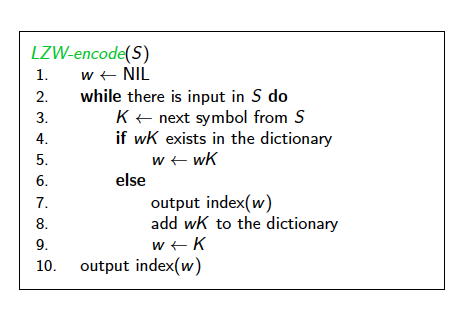
\includegraphics[scale=0.7]{1}
\end{center}

\subsubsection*{LZW decoding}
\begin{center}
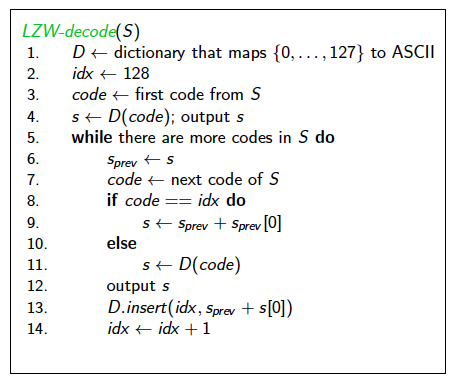
\includegraphics[scale=0.65]{2}
\end{center}

\subsection*{Compression summary}
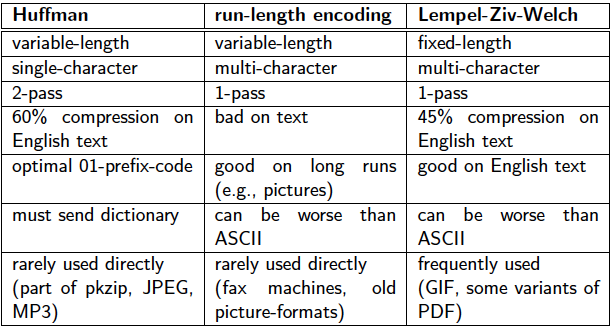
\includegraphics[scale=0.6]{3}

\subsection*{Text transformations}
For efficient compression, we need frequently repeating characters and/or frequently repeating substrings. 

\subsubsection*{Move-to-Front Encoding/Decoding}
\begin{center}
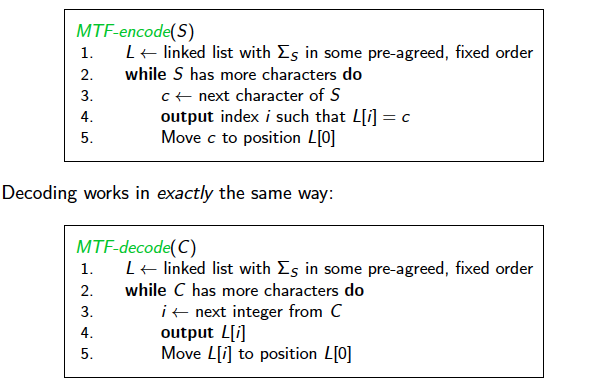
\includegraphics[scale=0.5]{4}
\end{center}

\subsection*{Burrows-Wheeler Transform}
The Burrows-Wheeler Transform is a sophisticated compression technique
\begin{itemize}
\item Transforms source text to a coded text with the same letters, just in a different order
\item The coded text will be more easily compressible with MTF
\item Compression algorithm does not make just a few "passes" over S. BWT is a block compression method.
\item Decoding is more efficient than encoding,
so BWT is an asymmetric scheme.
\end{itemize}

\subsubsection*{BWT Encoding}
A cyclic shift of a string X of length n is the concatenation of \(X[i + 1, \ldots, n -1]\) and \(X[0, \ldots 1]\) for \(0 \leq i \leq n\). 


For Burrows-Wheeler, we assume the source text S ends with a special
end-of-word character \$ that occurs nowhere else in S.


The Burrows-Wheeler Transform proceeds in three steps:
\begin{enumerate}
\item Place all cyclic shifts of S in a list L
\item Sort the strings in L lexicographically
\item C is the list of trailing characters of each string in L
\end{enumerate}

\subsubsection*{BWT Decoding}
View the coded text C as an array of characters
\begin{itemize}
\item Make array of A of tuples (C[i ]; i)
\item Sort A by the characters, record integers in array N
(Note: C[N[i ]] follows C[i ] in S, for all \(0 \leq i \leq n\))
\item Set j to index of \$ in C and S to empty string
\item  Set j   N[j ] and append C[j ] to S
\item Repeat Step 4 until C[j ] = \$
\end{itemize}

\subsubsection*{BWT Overview}
\textbf{Encoding Cost :} \(O(n^2)\) (using radix sort)
\begin{itemize}
\item Sorting cyclic shifts is equivalent to sorting suffixes
\item This can be done by traversing suffix trie
\item Possible in O(n) time
\end{itemize}
\textbf{Decoding cost :} \(O(n)\) (faster than encoding) 


Encoding and decoding both use \(O(n)\)


\section{External Memory}

Different levels of memory
\begin{itemize}
\item registers
\item cache L1, L2
\item main memory 
\item external memory 
\end{itemize}

\subsection*{Dictionaries in external memory}
Tree-based data structures have poor memory locality:
If an operation accesses m nodes, then it must access
m spaced-out memory locations.
\begin{itemize}
\item In an AVL tree, \(\theta(\log n)\) pages are loaded in the worst case
\item Better solution : B-trees
\end{itemize}

\subsection*{2-3 Trees}
A 2-3 tree is like a BST with additional structural properties 
\begin{itemize}
\item Every internal node either contains one KVP and two children,
or two KVPs and three children.
\item The leaves are NULL (do not store keys)
\item All the leaves are at the same level.
\end{itemize} 
Searching through a 1-node is just like in a BST.
For a 2-node, we must examine both keys and follow the appropriate path.

\subsubsection*{Insertion in a 2-3 Tree}
First, we search to find the lowest internal node where the new key
belongs.



If the node has only 1 KVP, just add the new one to make a 2-node.



Otherwise, otherwise order the three keys as \(a < b < c\). \\
split the node into two 1-nodes, containing a and c, and recursively insert b into the parent along with the new link.  

\subsubsection*{Deletion from a 2-3 Tree}
As with BSTs and AVL trees, we first swap the KVP with its successor,
so that we always delete from a leaf.


Say we're deleting KVP x from a node V:
\begin{itemize}
\item If V is a 2-node, just delete x.
\item ElseIf V has a 2-node immediate sibling U, perform a transfer :
Put the "intermediate" KVP in the parent between V and U into V,
and replace it with the adjacent KVP from U.
\item Otherwise, we merge V and a 1-node sibling U:
Remove V and (recursively) delete the "intermediate" KVP
from the parent, adding it to U.
\end{itemize}


\subsection*{B-trees}
The 2-3 Tree is a specific type of (a,b)-tree :

An \textbf{(a,b)-tree of order M} is a search tree satisfying 
\begin{itemize}
\item Each internal node has at least a children, unless it is the root.
The root has at least 2 children.
\item Each internal node has at most b children.
\item If a node has k children, then it stores k 􀀀 1 key-value pairs (KVPs).
\item Leaves store no keys and are at the same level.
\end{itemize}

A B-tree of order M is a \((ceiling(M/2), M)\) - tree. \\
A 2-3 tree has a M = 3. 

\subsubsection*{Height of a B-tree}
$$ \text{Total : } n \geq 1 + 2 \sum_{i=0}^{h-1} (M/2)^i (M/2-1) = 2(M/2)^h - 1$$
Therefore height of tree with n nodes is \(\theta((\log n ) / (\log M))\)

\subsubsection*{Analysis of B-tree operations}
Assume each node stores its KVPs and child-pointers in a dictionary that supports \(O(\log M)\) search, insert, and delete. 

Then search, insert, and delete work just like for 2-3 trees, and each
require \(\theta(height)\) node operations.

$$ \text{Total cost is } O\left(\frac{\log n}{\log M} \cdot (\log M)\right) = O(\log n) $$

\subsubsection*{B-tree variations}
\textbf{Other strategies:} insert and delete without backtracking via pre-emptive splitting and pre-emptive merging. \\
\textbf{Red-black trees:} identical to a B-tree with minsize 1 and maxsize 3, but each 2-node or 3-node is represented by 2 or 3 binary nodes, and each nodes holds a "color" value of red or black. \\
\textbf{B+ trees} : All KVPs are stored at the leaves (interior nodes just have keys) and the leaves are linked sequentially. 


\subsection*{Hashing in External Memory}
Compared to Linear probing, \textbf{Extendible Hashing} which is similar to a B-tree with height 1 and max size S at the leaves is a more efficient approach. 

\subsubsection*{Extendible Hashing Overview}
\begin{itemize}
\item The \textbf{directory} (similar to root node) is stored in \textbf{internal memory} . Contains array of size \(2^d\), where \(d \leq L\) is called the order .
\item Each directory entry points to a \textbf{block} stored in external memory. Each block contains at most S items. 
\item To look up a key k in the directory use the d leading bits of h(k).
\end{itemize}

\subsubsection*{Extendible Hashing Details}
Blocks are shared by entries in a specific manner 
\begin{itemize}
\item Every block B stores a \textbf{local depth} \(k_B \leq d\).
\item Hash values in B agree on leading \(k_B\) bits
\item All directory entries with the same \(k_B\) leading bits point to B
\item So \(2^{d-k_N}\) directory entries point to a block B 
\end{itemize}

\subsubsection*{Searching in Extendible Hashing}
Searching is done in the directory, then in a block:
\begin{itemize}
\item Given a key k, compute h(k).
\item Leading d digits of h(k) give index in directory.
\item Load block B at this index into main memory.
\item Perform a search in B for all items with hash value h(k).
\item Search among them for the one with key k.
\end{itemize}
\textbf{Cost:}
\begin{itemize}
\item CPU  time : depends on how the blocks are organized
\item Disk transfers : 1 (directory resides in internal memory)
\end{itemize}

\subsubsection*{Insertion in Extendible Hashing}
\begin{center}
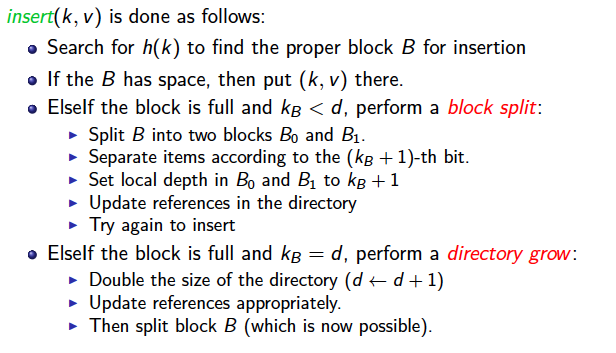
\includegraphics[scale=0.7]{5}
\end{center}

\subsubsection*{Extendible hashing conclusion}
\begin{center}
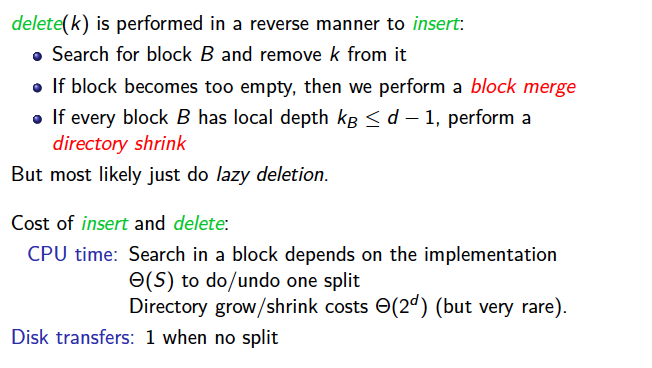
\includegraphics[scale=0.7]{6}
\end{center}

\subsubsection*{Summary of Extendible Hashing}
\begin{itemize}
\item Directory is much smaller than total number of stored keys and
should fit in main memory.
\item To make more space, we only add one block.
Rarely do we have to change the size of the directory.
Never do we have to move all items in the dictionary
(in contrast to normal hashing).
\item Space usage is not too inefficient: can be shown that
under uniform hashing, each block is expected to be 69% full.
\item Potentially extra CPU cost
\end{itemize}


\end{document}
